

%\documentclass[12pt]{article}
\documentclass[12pt, tikz]{scrartcl}
\nonstopmode
%\usepackage[utf-8]{inputenc}
\usepackage{graphicx} % Required for including pictures
\usepackage[figurename=Figure]{caption}

\usepackage{float}    % For tables and other floats
\usepackage{pstricks-add}
\usepackage{verbatim} % For comments and other
\usepackage{parallel,enumitem} % For split pages
\usepackage{amsmath}  % For math
\usepackage{amssymb}  % For more math
\usepackage{fullpage} % Set margins and place page numbers at bottom center
\usepackage{paralist} % paragraph spacing
\usepackage{listings} % For source code
\usepackage{subfig}   % For subfigures
%\usepackage{physics}  % for simplified dv, and 
\usepackage{enumitem} % useful for itemization
\usepackage{siunitx}  % standardization of si units
\usepackage{mathtools}
\usepackage{tikz,bm} % Useful for drawing plots
%\usepackage{tikz-3dplot}
\usepackage{circuitikz}
\usepackage{pgfplots}
\usepgfplotslibrary{polar} %plot polat axis
\usetikzlibrary{decorations.pathreplacing,bending}
\usepgfplotslibrary{fillbetween}
\usepackage{esvect}
\newcommand{\AxisRotator}[1][rotate=0]{%
    \tikz [x=0.25cm,y=0.60cm,line width=.2ex,-stealth,#1] \draw (0,0) arc (-150:150:1 and 1);%
}
\allowdisplaybreaks %Allow page breaks 

\begin{document}


\begin{center}
	\hrule
	\vspace{.4cm}
	{\textbf { \large ECE241, PRA0105 - Digital Logic}}
\end{center}
{\textbf{Name:}\ Christina Pizzonia \hspace{\fill} \textbf{Due Date:}  19 September, 2023}   \\
{ \textbf{Student Number:}} \ 1007914250 \hspace{\fill} \textbf{Prelab:} Number 1 \\
	\hrule
\usetikzlibrary{intersections, angles, quotes} % For triangles

\section*{Part I}
\paragraph*{1. Multiplexer schematic diagram} \hfill \newline
This diagram illustrates the resultant function $ f = \bar s x + xy$. 
\begin{figure}[hp]
\begin{center}
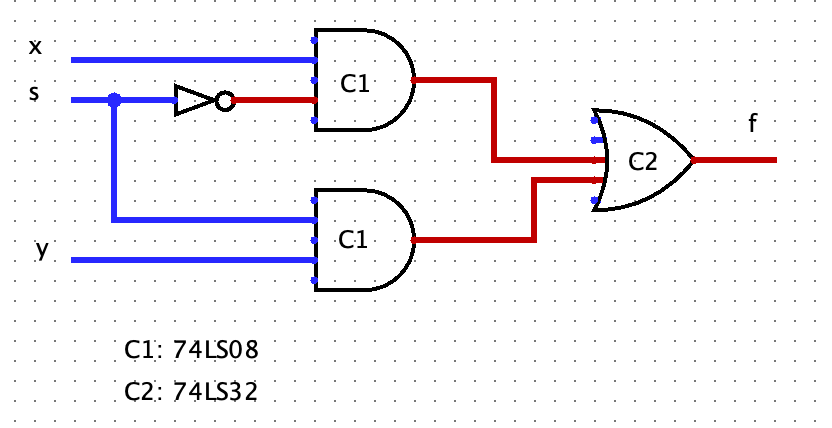
\includegraphics[width=9cm]{q1.png}
\end{center}
\end{figure}
Note: 
\begin{itemize}
	\item 7404: Not
	\item 7408: And
	\item 7432: Or
\end{itemize}
\paragraph*{2. Truth table} \hfill \newline
\begin{table}[h]
	\centering
	\begin{tabular}{|c|c|c||c|}
	\hline
	x & s & y & $f = x\bar s + ys$ \\ \hline
	0 & 0 & 0 & 0 \\ \hline
	0 & 0 & 1 & 0 \\ \hline
	0 & 1 & 0 & 0 \\ \hline
	0 & 1 & 1 & 1 \\ \hline
	1 & 0 & 0 & 1 \\ \hline
	1 & 0 & 1 & 1 \\ \hline
	1 & 1 & 0 & 0 \\ \hline
	1 & 1 & 1 & 1 \\ \hline
	\end{tabular}
	\end{table}

\newpage
\paragraph*{3. Logisim schematic and simulation output} \hfill \newline
\begin{figure}[hp]
\begin{center}
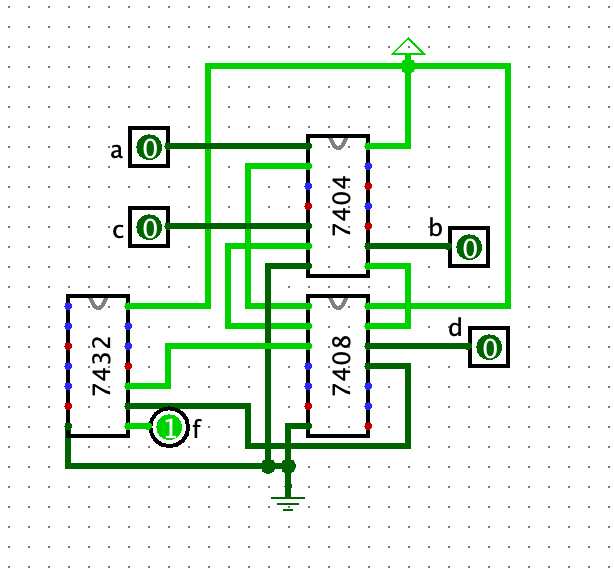
\includegraphics[width=9cm]{q22.png}
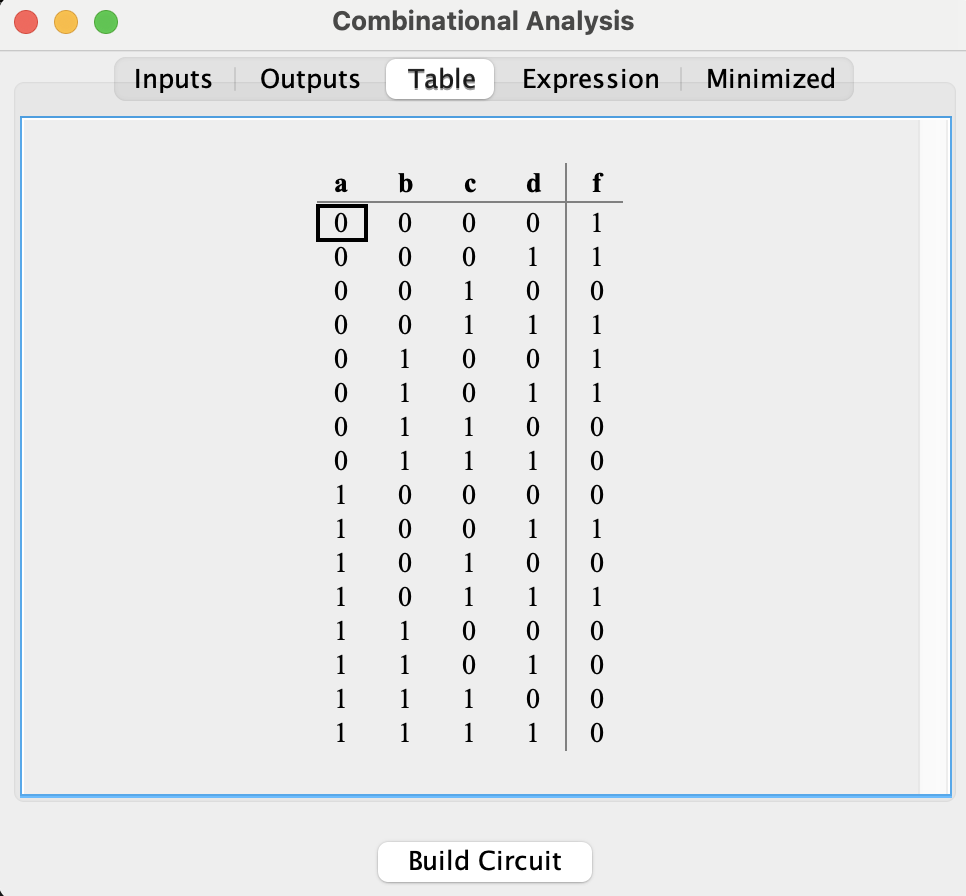
\includegraphics[width=9cm]{q21.png}
\end{center}
\end{figure}

\paragraph*{4. Cheaper implementation} \hfill \newline
No, there is no cheaper implementation (i.e. expression cannot be simpliified using Boolean algebra).

\section*{Part II}
\paragraph*{6. Simpler implementation} \hfill \newline
\paragraph*{1. Schematic} \hfill \newline
\paragraph*{2. Truth table} \hfill \newline
\paragraph*{3. Logisim schematic and simulation output} \hfill \newline
\end{document} 


